\chapter{Implementación}


\section{Controladores}

El controlador digital presentado en la sección \ref{cap3_controladores} se implementó en lenguaje C usando la transformada directa II.

%https://www.keil.com/pack/doc/CMSIS/DSP/html/group__BiquadCascadeDF2T.html


\subsection{Microcontrolador}



\subsection{Puente H}

Funciones especificas

\section{Integración de hardware}

Esquematico y componentes

\subsubsection{PCB}

Placa PCB

\section{Bus de campo}

Conexión


\section{Software}

\subsection{ROS}

Como se monstró en el capitulo pasado, su utilizó ROS como framework para realizar la integración. Los dispositivos de hardware, el robot Scorbot y el dispotivo háptico Phantom, cuentan con su \textit{nodo driver} que permiten la integración con el ecosistema ROS.

Se entiende por \textit{nodo driver} o ROS \textit{wrapper}, a una aplicación que actua como puente entre un dispositivo fisico y su representación en ROS, permitiendo interactuar de forma transparente con el dispositivo mediante el uso tópicos y servicios. Usualmente el \textit{nodo driver} hace uso de librerías proveidas por el fabricante o terceros para el manejo protocolos especificos del dispositivo. Por ejemplo, las siguientes aplicaciones cumplen esta función:

\begin{itemize}

\item \textit{ROSARIA}\cite{rosaria}: corresponde a una aplicación construido usando la librería \textit{Adept MobileRobots Robotics Interface for Applications} (ARIA), permite el control de robots móviles de las compañias Adept MobileRobots, MobileRobots Inc., y ActivMedia, por ejemplo el Pioneer 3-DX y 3-AT.

\item \textit{kinova-ros}\cite{kinova}: Es el driver oficial ofrecido por Kinova robotics para el uso de los robot manipuladores Jaco y Mico.

\end{itemize}

\subsubsection{Integración del robot Scorbot}

En esta sección se describirá la función de cada uno de los nodos que integran el software desarrollado para el control del robot Scorbot.

\begin{figure}[ht]
  \centering
  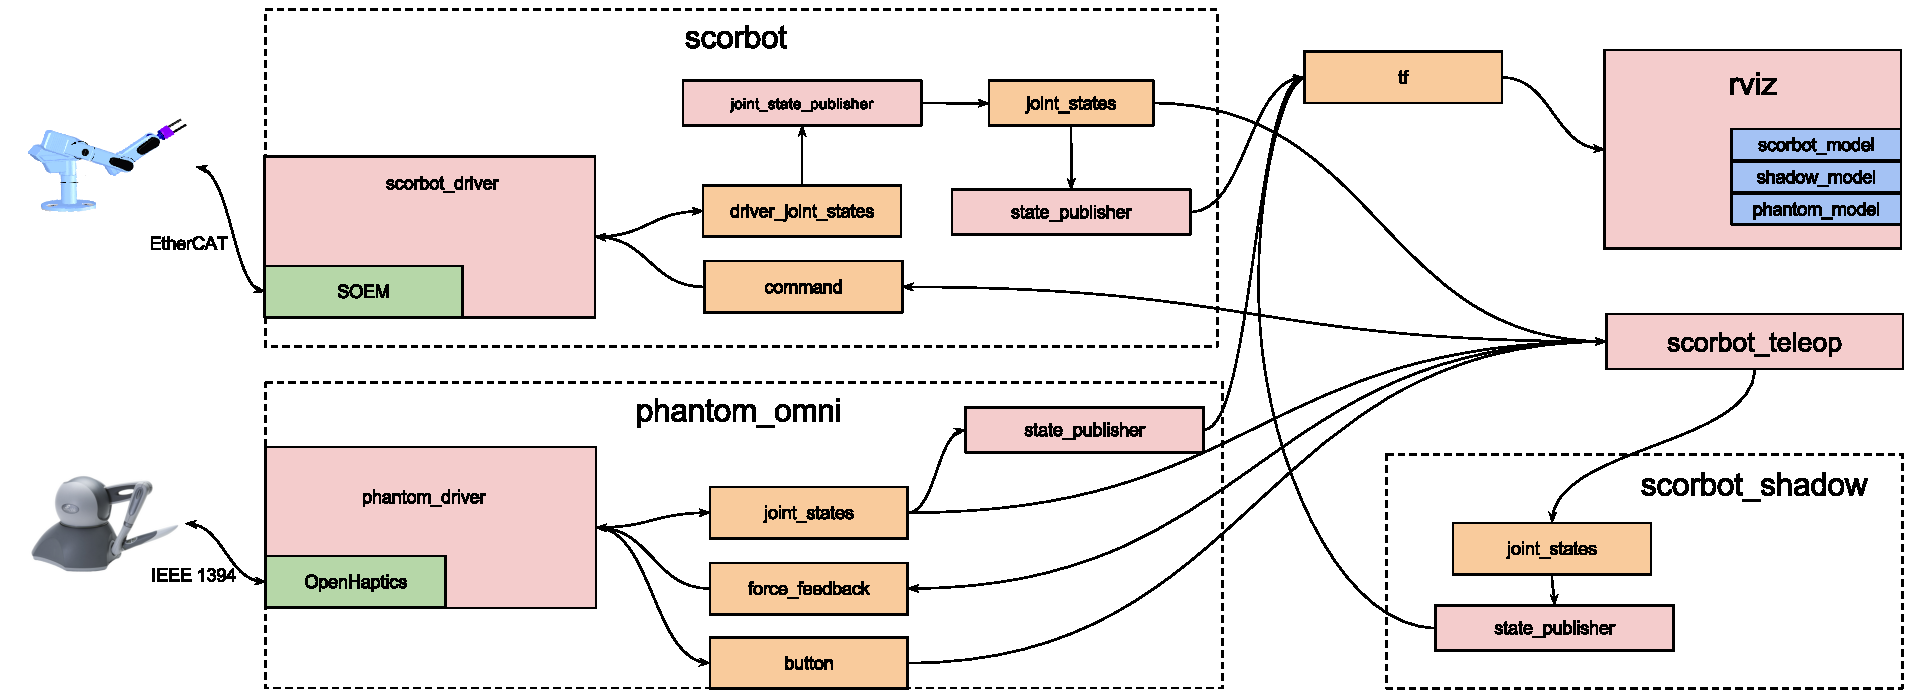
\includegraphics[width=\textwidth]{img/cap4/scorbot_software.pdf}
  \caption{Diagrama de nodos y tópicos de la aplicación.}
  \label{cap4_scorbot_software}
\end{figure}

\begin{description}

\item[\texttt{scorbot\_driver}] Corresponde al \textit{nodo driver} se integra con la librería SOEM \cite{soem} para la comunicación EtherCAT.

\end{description}


La integración principal con el robot Scorbot se realiza en el nodo 



